
   %%%%%%%%%%%%%%%%%%%%%%%
 %%%  NOAH'S SUPER COOL  %%%
%%%%      ACADEMIC       %%%%
 %%%   LATEX TEMPLATE    %%%
   %%%%%%%%%%%%%%%%%%%%%%%

\documentclass[12pt]{article}
\usepackage[letterpaper]{geometry}
\geometry{top=1in, bottom=1in, left=1in, right=1in}
\usepackage{fontspec}
\usepackage{tgtermes}
\usepackage{hanging}
\setmainfont[
 ItalicFont={texgyretermes-italic.otf},
 BoldFont={texgyretermes-bold.otf},
 ]{texgyretermes-regular.otf}
\usepackage{setspace}
\doublespacing
\usepackage{graphicx}
\graphicspath{ {./graphics/} }

\begin{document}

% Title Page
\pagenumbering{gobble} % remove page numbers
\begin{center}
\topskip0pt
\vspace*{\fill}
Momentum and Energy in Collisions Lab 9 \\ Noah Dinan \\ PHY 1110 - Mayer \\ \today \\
\vspace*{\fill}
\end{center}

\newpage
\pagenumbering{arabic} % resume page numbering
\setlength{\parindent}{0in}

\textbf{Results}

In this lab report, we examined both elastic and inelastic collisions and the
Law of Conservation of Linear Momentum which states that \textbf{the total momentum
of a system remains constant if there is no net external force acting on the system}.

A major potential source of experimental error was any small amounts of friction that may
have been present despite using the air track.

For the elastic collision, after the collision we noticed that the first sled moved after the collision
very slightly. We believe this was due to the uneven balance of the air track and recorded the momentum for that
sled to be 0.


The equation for momentum is
\[ \vec{p} = m\vec{v} \]


We measured the mass for the cart to be $184.3$ grams and the width of the flag to be $2.95$ centimeters.
Using this equation for momentum, we filled the below table for an elastic collision.

\begin{center}
   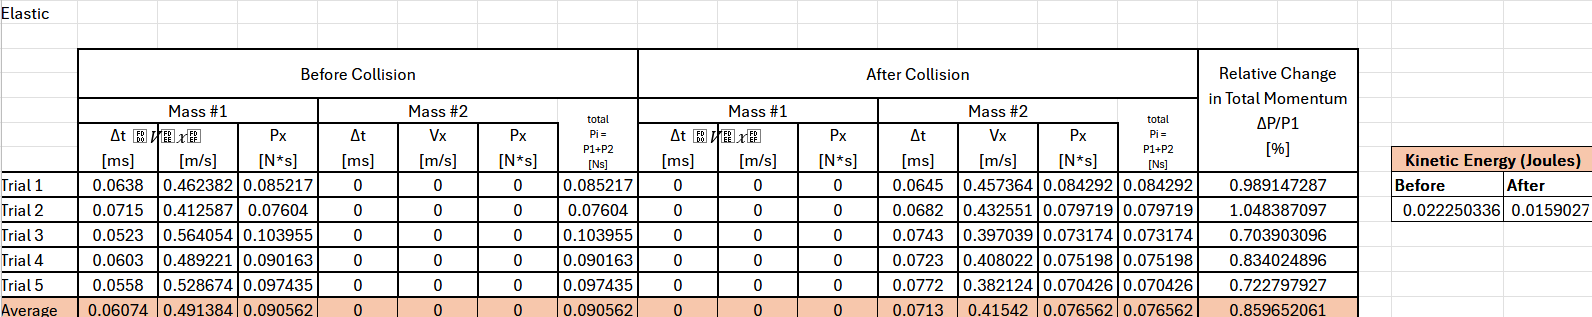
\includegraphics[scale=0.5]{elastic_1.png}
\end{center}

We then repeated the experiment for an inelastic collision to create the following table.

\begin{center}
   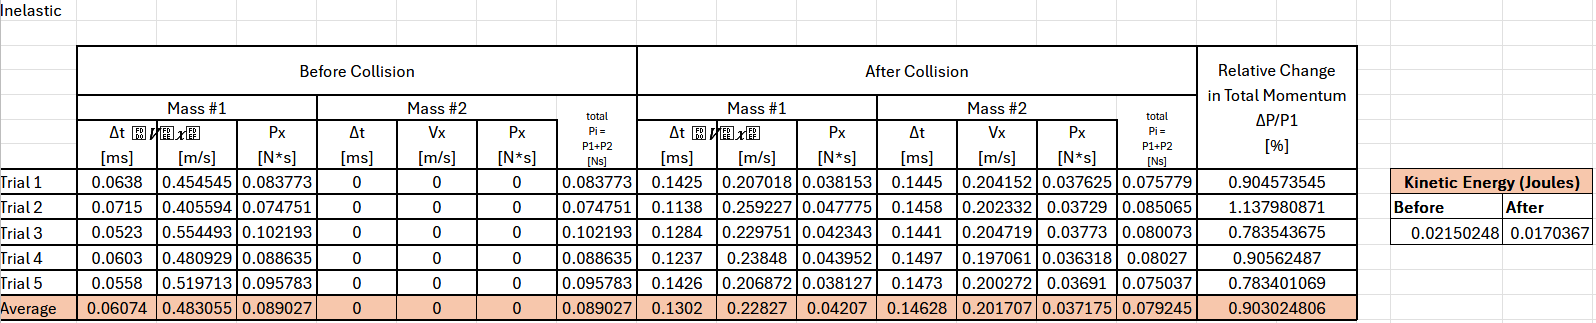
\includegraphics[scale=0.5]{inelastic_1.png}
\end{center}

After completing our first trial for elastic and inelastic collisions, we performed two more trials
altering the mass of the sleds. The data tables for trials two and three are shown below

\textbf{Trial 2}
\begin{center}
   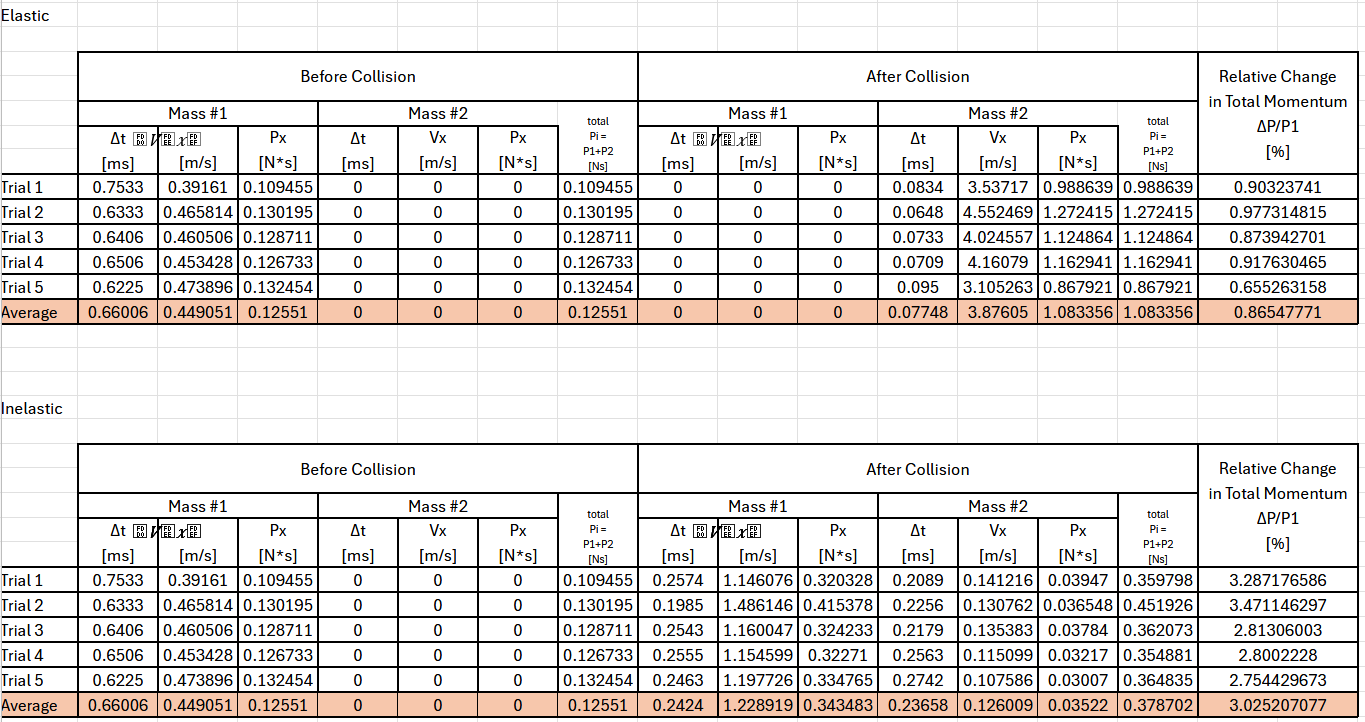
\includegraphics[scale=0.6]{trial_2.png}
\end{center}

\textbf{Trial 3}
\begin{center}
   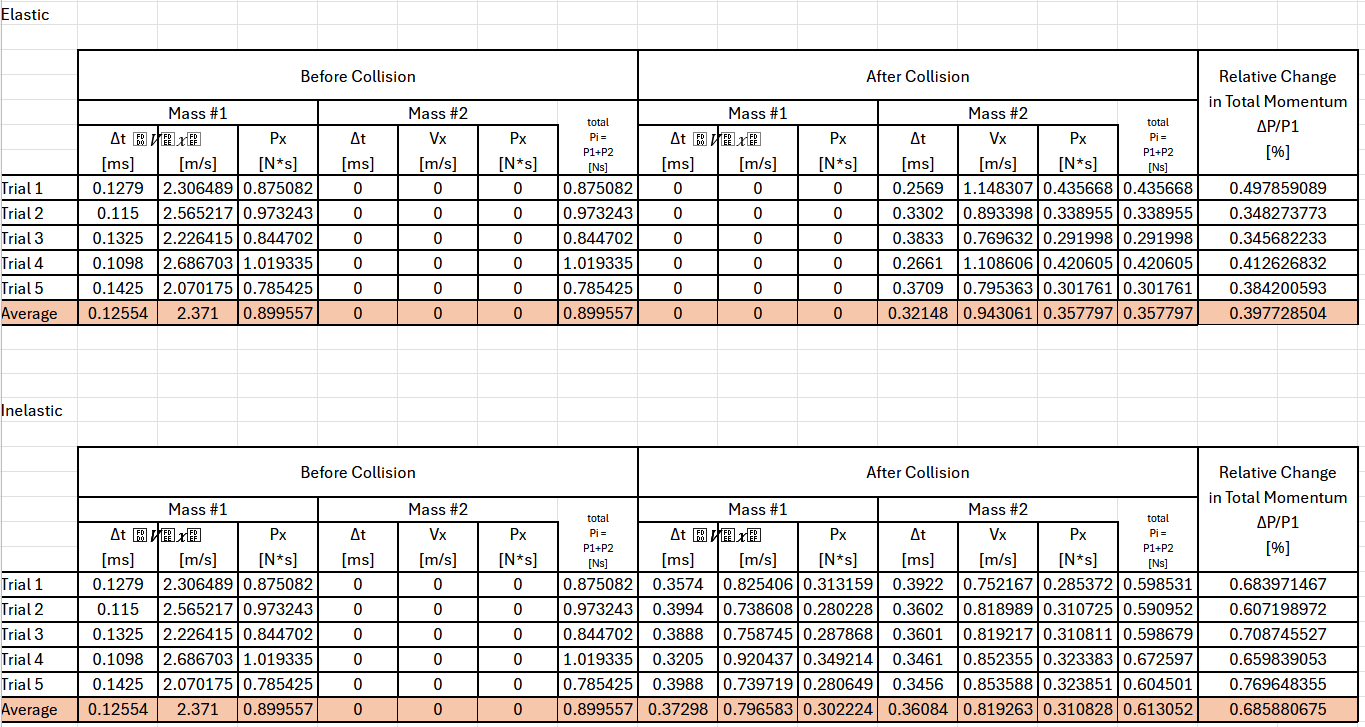
\includegraphics[scale=0.6]{trial_3.png}
\end{center}

\newpage

\textbf{Conclusions}

Our results for this experiment were consistent with the Law of Conservation of Linear Momentum
as the differences between our momentum before and after collisions was fairly low (between 0.5 and 3\%).
For this reason I would also conclude that momentum \textbf{is} conserved for these collisions.

In addition, the change in kinetic energy before and after collisions (shown beside the tables for trial one),
is relatively low revealing that kinetic energy is conserved as well.

\end{document}
